\documentclass[12pt,a4paper]{article}
\usepackage[UTF8]{ctex} % 支持中文
\usepackage{geometry}
\usepackage{graphicx}
\usepackage{amsmath}
\usepackage{float}
\usepackage{subfigure}
\usepackage{booktabs} % 表格美化
\usepackage{cite}
\usepackage{ulem}
\usepackage{array}
\usepackage{multirow}

\newcolumntype{M}[1]{>{\centering\arraybackslash}m{#1}}
\newcommand{\down}[2]
{
	$#1_{#2}$
}

% 设置页面边距
\geometry{left=2.5cm,right=2.5cm,top=2.5cm,bottom=2.5cm}

\title{\Huge{\textbf{\uuline{实\ 验\ 报\ 告}}}}
\author{\uline{少年班}\ 学院 \quad 姓名:\ \uline{顾泓宇} \quad 学号:\ \uline{PB23000078} \quad 实验日期:\ \uline{2024-4-22} }
\date{}

\begin{document}
	\maketitle
	
	\section{实验题目}
	整流滤波
	
	\section{实验目的}
	了解交流信号的几个参数，学习整流滤波电路的基本工作原理及制作一台直流电源。
	
	\section{实验仪器}
	信号发生器，示波器，数字电压表（直流电压档、交流电压档），电阻箱，可变电容箱，面包板，整流二极管，电容，电阻，导线若干 
	
	\section{实验原理}
	整流电路的作用是把交流电转换成直流电，严格地讲是单方向大脉动直流电，而滤波电路的作用是把大脉动
	直流电处理成平滑的脉动小的直流电。\\
	\subsection{整流原理}
	利用二极管的单向导电性可实现整流。\\
	\hspace*{2em}(1)半波整流：利用单个二极管，交流电中和二极管导通方向相同的部分可以显示出来，如图 6.2.1-2。\\
	\hspace*{2em}(2)全波整流：利用四个二极管组成的桥式等结构，使交流电变的正负半周期信号都被应用，如图 6.2.1-3。\\
	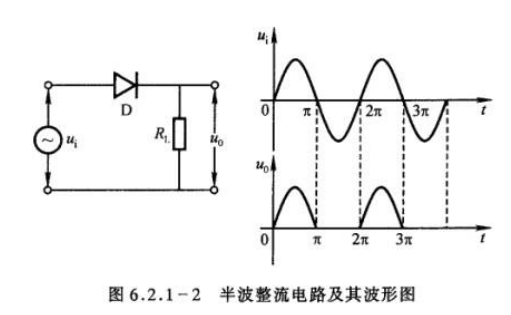
\includegraphics{电路1.png}
	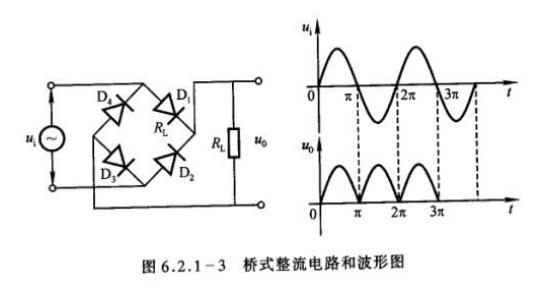
\includegraphics{电路2.png}\\
	
	\subsection{滤波原理}
	经过整流后的电压 (电流) 仍然是有“脉动”的直流电，为了减少波动，通常要加滤波器，常用的滤波电路
	有电容、电感滤波等。本实验使用电容滤波。  \\
	\hspace*{2em}(1) 单电容滤波：利用一个电容与负载并联，作为滤波，如图 6.2.1-4。\\
	\hspace*{2em}(2) $\pi$ 型电容滤波：即在单电容滤波基础上，在此之后又加了一级 RC 滤波，使得输出电压更平滑（但输出电压平均值要减少）。如图 6.2.1-6。\\
	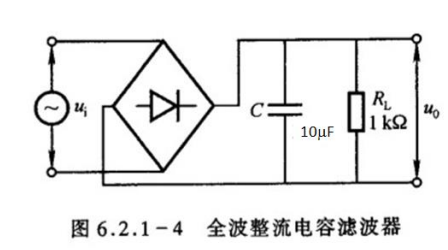
\includegraphics{电路3.png}
	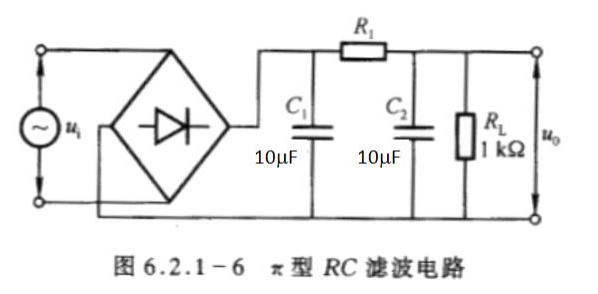
\includegraphics{电路4.png}\\
	\hspace*{2em}纹波系数是指负载上交流电压的有效值与直流电压之比，是表征直流电源品质的一个重要参数。除了与整流
	滤波电路品质有关之外，与外电路负载关系也很大。即：\\
	\begin{center}
		 纹波系数$K_u=\frac{\text{交流电压有效值}}{\text{直流电源}}\times 100\%$
	\end{center}
	
	
	\subsection{实验数据与处理、分析}
	\hangindent=1.3cm \hangafter=1
	\subsubsection{整流电路}
	\hspace*{2em} 如图1，2，3所示，分别为初始信号(10V,400Hz)、半波整流后的信号、全波整流后的信号的波形图。\\[14pt]
	\begin{minipage}{0.33\linewidth}
		\centering
		\textbf{图\ 1}\quad 初始信号波形图 \\[4pt]
		
\includegraphics[width=0.9\linewidth]{1.jpg}
		\label{tp5.png} 
	\end{minipage}
	\begin{minipage}{0.33\linewidth}
		\centering
		\textbf{图\ 2}\quad 半波整流波形图 \\[4pt]
		
\includegraphics[width=0.9\linewidth]{2.jpg}
		\label{tp6.png}
	\end{minipage}
	\begin{minipage}{0.33\linewidth}
		\centering
		\textbf{图\ 3}\quad 全波整流波形图 \\[4pt]
		
\includegraphics[width=0.9\linewidth]{3.jpg}
		\label{tp7.png}
	\end{minipage}
	\subsubsection{滤波电路}
	\hspace*{2em} 如图4, 5所示，分别为全波整流后的电流经过单电容($1\mu F$)滤波、$\pi$型电容($1\mu F\times 2$)滤波后的波形图。\\[14pt]
	\begin{minipage}{0.5\linewidth}
		\centering
		\textbf{图\ 4}\quad 单电容($1\mu F$)滤波波形图 \\[4pt]
		
\includegraphics[width=0.9\linewidth]{4.jpg}
		\label{tp8.png}
	\end{minipage}
	\begin{minipage}{0.5\linewidth}
		\centering
		\textbf{图\ 5}\quad $\pi$型电容($1\mu F\times 2$)滤波波形图 \\[4pt]
		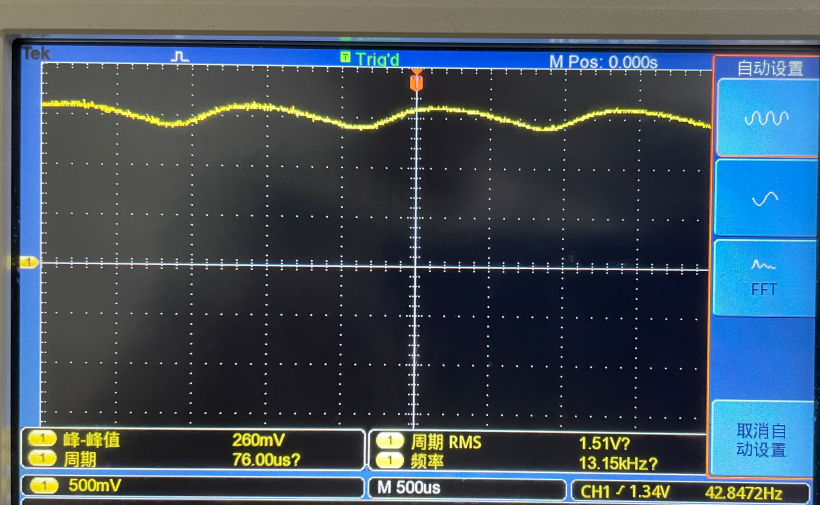
\includegraphics[width=0.9\linewidth]{pi型电容.png}
		\label{tp9.png}
	\end{minipage}\\[14pt]
	\hspace*{2em} 下表一为滤波后的直流电压和交流电压有效值，以及计算得到的纹波系数。
	\begin{center}
		\textbf{表\ 一}\quad $1\mu F$电容滤波数据  \\[4pt]
		\begin{tabular}{|c|c|c|c|}
			\hline
			滤波种类        & 直流电压/$V$   & 交流电压有效值/$V$  & 纹波系数  \\ \hline
			单电容滤波      & 2.543         & 0.567            & 22.2\% \\ \hline
			$\pi$型电容滤波 & 1.4859        & 0.0650            & 4.374\% \\ \hline
		\end{tabular}
	\end{center}
	\subsection{电容对滤波效果的影响}
	\hspace*{2em} 将上述所有$1\mu F$更改为$10\mu F$，重新测量直流电压和交流电压有效值，再计算纹波系数，
	波形如下图6，7，数据如下表二。\\[14pt]
	\begin{minipage}{0.5\linewidth}
		\centering
		\textbf{图\ 6}\quad 单电容($10\mu F$)滤波波形图 \\[4pt]
		
\includegraphics[width=0.9\linewidth]{5.jpg}
		\label{tp10.png}
	\end{minipage}
	\begin{minipage}{0.5\linewidth}
		\centering
		\textbf{图\ 7}\quad $\pi$型电容($10\mu F\times 2$)滤波波形图 \\[4pt]
		
\includegraphics[width=0.9\linewidth]{6.jpg}
		\label{tp11.png}
	\end{minipage}
	\begin{center}
		\textbf{表\ 二}\quad $10\mu F$电容滤波数据  \\[4pt]
		\begin{tabular}{|c|c|c|c|}
			\hline
			滤波种类        & 直流电压/$V$   & 交流电压有效值/$V$  & 纹波系数  \\ \hline
			单电容滤波      & 2.954         & 0.0745            & 2.522\% \\ \hline
			$\pi$型电容滤波 & 1.6089        & 0.0001            & 0.006\% \\ \hline
		\end{tabular}
	\end{center}
	波形差异：和1$\mu F$相比，整体波形更加平滑，但输出电压平均值有所下降。\\
	分析解释：和1$\mu F$相比，电容增大，电容充放电能力、蓄电能力增强，则对于电路的交流部分削弱的更明显，
	即交流部分更小，同时直流部分也有所增加，所以纹波系数更小。
	
\section{思考题}
1. 整流、滤波的主要目的是什么?\\
\hspace*{2em}答：把交流电源改为直流电源。可以使电流更加的稳定，供一般的电路使用。\\
\hspace*{2em}2. 滤波电路中电容是否越大越好？请根据实验过程简述理由。\\
\hspace*{2em}答：不是，虽然理想的状态下可以认为电容越大会使纹波系数更小，但是实际实验中当电容变大时，电压会减小，产生大量的能源浪费，且可能使电压达不到实际使用要求，使得电路可用性变低。
	
	
\end{document}

